\documentclass[10pt,aspectratio=169]{beamer}

%\documentclass[fleqn,aspectratio=169]{beamer}

\usepackage{amsmath, amssymb}
\usepackage{fancyvrb, color, graphicx, hyperref, url}

%\setbeamersize{text margin left=5pt, text margin right=5pt}

\setlength{\parskip}{\smallskipamount}
\setlength{\parindent}{0pt}

\usepackage{fontspec}
%\setmonofont{DejaVu Sans Mono}
\setmonofont{JuliaMono-Regular}

\usefonttheme[onlymath]{serif}

\usepackage{minted}
\newminted{python}{breaklines,fontsize=\footnotesize}
\newminted{julia}{breaklines,fontsize=\footnotesize}
\newminted{bash}{breaklines,fontsize=\footnotesize}
\newminted{text}{breaklines,fontsize=\footnotesize}

\newcommand{\txtinline}[1]{\mintinline[breaklines,fontsize=\footnotesize]{text}{#1}}
\newcommand{\pyinline}[1]{\mintinline[breaklines,fontsize=\footnotesize]{python}{#1}}
\newcommand{\jlinline}[1]{\mintinline[breaklines,fontsize=\footnotesize]{julia}{#1}}

\definecolor{mintedbg}{rgb}{0.95,0.95,0.95}
\usepackage{mdframed}

\BeforeBeginEnvironment{minted}{\begin{mdframed}[backgroundcolor=mintedbg,%
  rightline=false,leftline=false,topline=false,bottomline=false]}
\AfterEndEnvironment{minted}{\end{mdframed}}

% https://tex.stackexchange.com/questions/33969/changing-font-size-of-selected-slides-in-beamer

\usepackage{environ}
%
% Custom font for a frame.
%
\newcommand{\customframefont}[1]{
  \setbeamertemplate{itemize/enumerate body begin}{#1}
  \setbeamertemplate{itemize/enumerate subbody begin}{#1}
}

\NewEnviron{framefont}[1]{
  \customframefont{#1} % for itemize/enumerate
  {#1 % For the text outside itemize/enumerate
    \BODY
  }
  \customframefont{\normalsize}
}



\begin{document}

\title{Density Functional Theory Calculations for 1d Systems}
\author{Fadjar Fathurrahman}
\institute{
Teknik Fisika \\
Institut Teknologi Bandung
}
\date{}


\frame{\titlepage}


\begin{frame}
\frametitle{Introduction: Kohn-Sham equations (in 3d)}

\begin{equation*}
\mathcal{H}_{\mathrm{KS}} \psi_{i}(\mathbf{r}) = \epsilon_{i} \psi_{i}(\mathbf{r})
\end{equation*}

\begin{equation*}
\mathcal{H}_{\mathrm{KS}} =
-\frac{1}{2} \nabla^2 +
V_{\mathrm{ion}}(\mathbf{r}) +
V_{\mathrm{H}}(\mathbf{r}) + V_{\mathrm{xc}}(\mathbf{r})
\end{equation*}

\end{frame}


\begin{frame}
\frametitle{Electron density, Hartree and XC potentials}

\begin{equation*}
\rho(\mathbf{r}) = \sum_{i} f_{i} \psi_{i}(\mathbf{r}) \psi^{*}_{i}(\mathbf{r}) 
\end{equation*}

\begin{equation*}
V_{\mathrm{H}}(\mathbf{r}) = \int \frac{\rho(\mathbf{r}')}{\left| \mathbf{r} - \mathbf{r}' \right|}
\,\mathrm{d}\mathbf{r}'
\end{equation*}

\begin{equation*}
V_{\mathrm{xc}}(\mathbf{r}) = \frac{\delta E_{\mathrm{xc}}[\rho(\mathbf{r})]}%
{\delta \rho(\mathbf{r})}
\end{equation*}

\end{frame}



\begin{frame}
\frametitle{Self-consistency}

\begin{itemize}
\item Some terms of $\mathcal{H}_{\mathrm{KS}}$ depends on $\rho(\mathbf{r})$.
To calculate its matrix elements we need to know $\rho(\mathbf{r})$.
\item To calculate $\rho(\mathbf{r})$, we need to know $\psi_{i}(\mathbf{r})$
\item To calculate $\psi_{i}(\mathbf{r})$, we need to diagonalize $\mathcal{H}_{\mathrm{KS}}$
\end{itemize}

Kohn-Sham equations need to be solved self-consistently.

\end{frame}


% -----------------------------
\begin{frame}
\frametitle{Simplified, 1d Kohn-Sham model}

\begin{equation*}
E_{\mathrm{KS}}[\psi_{i}(x)] = E_{\mathrm{kin}} + E_{\mathrm{ion}} +
E_{\mathrm{H}} + E_{\mathrm{xc}}
\end{equation*}

\begin{equation*}
E_{\mathrm{kin}} = -\frac{1}{2} \int \psi^{*}_{i}(x)
\frac{\mathrm{d}^2}{\mathrm{d}x^2} \psi_{i}(x) \, \mathrm{d}x
\end{equation*}


\begin{equation*}
E_{\mathrm{ion}} = \int \psi^{*}(x) V_{\mathrm{ion}} \psi_{i}(x) \, \mathrm{d}x
\end{equation*}

\begin{equation*}
E_{\mathrm{H}} = \frac{1}{2} \int \int \frac{\rho(x) \rho(x')}{\left| x - x' \right|}
\,\mathrm{d}x \,\mathrm{d}x'
\end{equation*}

\begin{equation*}
E_{\mathrm{xc}} = \int \varepsilon_{\mathrm{xc}}[\rho(x)]
\rho(x) \, \mathrm{d}x
\end{equation*}

\end{frame}



% -------------------------
\begin{frame}
\frametitle{Kohn-Sham equations}

\begin{equation*}
H_{\mathrm{KS}} \psi_{i}(x) = \epsilon_{i} \psi_{i}(x)
\end{equation*}

\begin{equation*}
H_{\mathrm{KS}} =
-\frac{1}{2} \frac{\mathrm{d}^2}{\mathrm{d}x^2} +
V_{\mathrm{ion}}(x) + V_{\mathrm{H}}(x) + V_{\mathrm{xc}}(x)
\end{equation*}


\begin{equation*}
V_{\mathrm{H}}(x) = \int \frac{\rho(x')}{\left| x - x' \right|} \,\mathrm{d}x'
\end{equation*}


\begin{equation*}
V_{\mathrm{xc}}(x) = \frac{\delta E_{xc}[\rho(x)] }{\delta \rho(x)}
\end{equation*}

\end{frame}



\begin{frame}
\frametitle{Solving Schroedinger equation}

Ignore Hartree and XC potential:
\begin{equation*}
\left[ -\frac{1}{2}\frac{\mathrm{d}^2}{\mathrm{d}x^2} + V_{\mathrm{ion}}(x) \right] \psi(x) = E\, \psi(x)
\end{equation*}
No need to do self-consistent calculation.

$V_{\mathrm{ion}}(x)$ can be any external potentials which do not depend on $\psi(x)$ or
$\rho(x)$ (otherwise we need to do self-consistent calculation).

\end{frame}


\begin{frame}
\frametitle{Boundary condition}

Assume the following boundary condition for wave function:
\begin{equation*}
\lim_{x \rightarrow \pm \infty} \psi(x) = 0
\end{equation*}

\end{frame}


\begin{frame}
\frametitle{Numerical solution of Schroedinger equation}

\begin{itemize}
\item basis set expansion (using plane wave basis set, Gaussian basis set, etc)
\item \textbf{finite-difference discretization}
\item finite-element
\item ...
\end{itemize}

\end{frame}



\begin{frame}
\frametitle{Finite difference approximation}

Discretize domain $[x_{\mathrm{min}},x_{\mathrm{max}}]$ using finite number
of points with equal spacing $\{ x_{i} \}$, $i = 1,2,\ldots,N$.

Approximate $\psi(x)$ using its values at these grid points. Stack them together
in a column vector.

\begin{equation*}
\psi(x) \rightarrow
\begin{bmatrix}
\psi(x_{1}) \\ \psi(x_{2}) \\ \cdots \\ \psi(x_{N})
\end{bmatrix}
\end{equation*}

\end{frame}



\begin{frame}[fragile]
\frametitle{Real-space discretization}

We will make a grid of points in $x$ axis.
\begin{juliacode}
function init_FD1d_grid( x_min::Float64, x_max::Float64, N::Int64 )
    L = x_max - x_min
    h = L/(N-1)
    x = zeros(Float64,N)
    for i = 1:N
        x[i] = x_min + (i-1)*h
    end
    return x, h
end
init_FD1d_grid( X, N ) = init_FD1d_grid( X[1], X[2], N )
\end{juliacode}

\end{frame}


\begin{frame}[fragile]
\frametitle{Example discretization}

Suppose that we want to discretize $x$ domain from $x_{\mathrm{min}} = -8.0$
to $x_{\mathrm{max}} = 8.0$ with 9 points.
We call \pyinline{init_FD1d_grid} as:
\begin{juliacode}
xgrid, dx = init_FD1d_grid(-8.0, 8.0, 9)
\end{juliacode}

Result \jlinline{xgrid}:
\begin{textcode}
[-8.0, -6.0, -4.0, -2.0, 0.0, 2.0, 4.0, 6.0, 8.0]
\end{textcode}

Result \jlinline{dx}:
\begin{textcode}
2.0
\end{textcode}

\end{frame}


\begin{frame}[fragile]
\frametitle{Gaussian function}

\begin{equation*}
f(x) = e^{-\alpha x^2}
\end{equation*}

Take $\alpha = 1$.

Plot this function using discretized points on interval $[-5, 5]$.

Try various number of grid points.

\begin{juliacode}
function my_gaussian(x; α=1.0)
    return exp(-α*x^2)
end
\end{juliacode}

Note that we use default value of $\alpha = 1$. Try using different value of $\alpha$.

\end{frame}


% -----------------------------------------------
\begin{frame}[fragile]

\begin{juliacode}
A = -5.0; B =  5.0
xgrid, dx = init_FD1d_grid( A, B, N )
fx = my_gaussian.(xgrid)

Ndense = 200 # for reference
x_dense = range(A, stop=B, length=Ndense)
fx_dense = my_gaussian.(x_dense)

plt.clf()
plt.plot(xgrid, fx, marker="o", label=L"Sampled $f(x)$")
plt.plot(x_dense, fx_dense, label=L"f(x)")
plt.legend()
plt.grid()
plt.title(plot_title)
plt.savefig("IMG_gaussian_f_"*string(N)*".pdf")
\end{juliacode}

\end{frame}


% ------------------
\begin{frame}

{\centering
\includegraphics[width=0.8\textwidth]{../../codes/ks_dft_1d/IMG_gaussian_f_15.pdf}
\par}

\end{frame}


\begin{frame}

{\centering
\includegraphics[width=0.8\textwidth]{../../codes/ks_dft_1d/IMG_gaussian_f_51.pdf}
\par}

\end{frame}


\begin{frame}[fragile]
\frametitle{Approximating integral}

\begin{equation*}
I = \int e^{-\alpha x^2}\, \mathrm{d}x = \sqrt{ \frac{\pi}{\alpha} }
\end{equation*}
\begin{equation*}
I \approx \sum_{i} e^{-\alpha x_{i}^2} \Delta x
\end{equation*}

\begin{juliacode}
function do_integrate(N::Int64)
    A = -5.0
    B = 5.0
    α = 1.0
    xgrid, dx = init_FD1d_grid( A, B, N )
    fx = my_gaussian.(xgrid, α=α)
    exact_res = sqrt(π)/sqrt(α)
    num_res = sum(fx)*dx # approximate the integral
    @printf("%5d %18.10f %10.5e\n", N, num_res, abs(exact_res - num_res))
end

for N in [10, 20, 30, 40, 50]
    do_integrate(N)
end
\end{juliacode}

\end{frame}



% ---------------------------------------------
\begin{frame}
\frametitle{Approximating 2nd derivative operator}

We approximate the 2nd order derivative operator using 3-points finite difference
formula:
\begin{equation*}
\frac{\mathrm{d}^2}{\mathrm{d}x^2} \psi_{i} =
\frac{\psi_{i+1} - 2\psi_{i} + \psi_{i-1}}{h^2}
\end{equation*}

Writing this out for $i = 1,2,\ldots,N$:
\begin{align*}
\psi''_{1} & \approx \left( \psi_{2} - 2\psi_{1} + \psi_{0} \right)/h^2 \\
\psi''_{2} & \approx \left( \psi_{3} - 2\psi_{2} + \psi_{1} \right)/h^2 \\
\psi''_{3} & \approx \left( \psi_{4} - 2\psi_{3} + \psi_{2} \right)/h^2 \\
& \vdots \\
\psi''_{N} & \approx \left( \psi_{N+1} - 2\psi_{N} + \psi_{N-1} \right)/h^2
\end{align*}

Thera are $\psi_{0}$ and $\psi_{N+1}$ in the above expression. They are outside
our domain (the points are numbered by $1,2,\ldots,N$ in our convention).

\end{frame}


\begin{frame}
\frametitle{Approximating 2nd derivative operator}

Assuming $\psi_{0} = 0$ and $\psi_{N+1} = 0$ we obtain:
\begin{align*}
\psi''_{1} & \approx \left( \psi_{2} - 2\psi_{1} \right)/h^2 \\
\psi''_{2} & \approx \left( \psi_{3} - 2\psi_{2} + \psi_{1} \right)/h^2 \\
\psi''_{3} & \approx \left( \psi_{4} - 2\psi_{3} + \psi_{2} \right)/h^2 \\
& \vdots \\
\psi''_{N} & \approx \left( - 2\psi_{N} + \psi_{N-1} \right)/h^2 \\
\end{align*}

\end{frame}


\begin{frame}
\frametitle{Matrix representation of 2nd derivative operator}

$\{ \psi \}$ and $\{ \psi'' \}$ represents discretized versions (column vectors)
of $\psi(x)$ and $\psi''(x)$, respectively.

\begin{equation*}
\{ \psi'' \} \approx \mathbb{D}^{(2)} \{ \psi \}
\end{equation*}

\begin{equation*}
\mathbb{D}^{(2)} = \frac{1}{h^2}
\begin{bmatrix}
-2  &  1  &  0  &  0  & 0 & \cdots & 0 \\
 1  & -2  &  1  &  0  & 0 & \cdots & 0 \\
 0  &  1  & -2  &  1  & 0 & \cdots & 0 \\
 \vdots  &  \ddots  &  \ddots  & \ddots  & \ddots  & \ddots & \vdots \\
 0 & \cdots & 0 & 1 & -2 & 1 & 0 \\
 0  &  \cdots  & \cdots & 0  & 1  & -2  & 1 \\
 0  &  \cdots  & \cdots & \cdots & 0  &  1  & -2 \\
\end{bmatrix}
\end{equation*}

\end{frame}


\begin{frame}
\frametitle{Testing 2nd derivative on a Gaussian function}

\begin{align*}
\psi(x) &= \mathrm{e}^{-\alpha x^2} \\
\psi''(x) &= \left( -2 \alpha + 4\alpha^2 x^2 \right) \mathrm{e}^{-\alpha x^2}
\end{align*}

\begin{itemize}
\item initialize column vector $\{ \psi \}$
\item initialize $D^{(2)}$ matrix
\item calculate approximation of $\psi''(x)$ by multiplying $D^{(2)}$ and $\{ \psi \}$
\item visualize the result
\end{itemize}

\end{frame}


\begin{frame}[fragile]

\begin{juliacode}
function build_D2_matrix_3pt( N::Int64, h::Float64 )
    mat = zeros(Float64,N,N)
    for i = 1:N-1
        mat[i,i] = -2.0
        mat[i,i+1] = 1.0
        mat[i+1,i] = 1.0
    end
    mat[N,N] = -2.0
    return mat/h^2
end
\end{juliacode}

\end{frame}


% ------------------------------------------
\begin{frame}[fragile]

\begin{juliacode}
function d2_my_gaussian(x; α=1.0)
    return (-2*α + 4*α^2 * x^2) * exp(-α*x^2)
end

A = -5.0; B =  5.0
x, h = init_FD1d_grid( A, B, N )
fx = my_gaussian.(x)
D2 = build_D2_matrix_3pt(N, h)
d2_fx_3pt = D2*fx

# For comparison
Ndense = 200 # choose sufficiently large number
x_dense = range(A, stop=B, length=Ndense)
fx_dense = my_gaussian.(x_dense)
d2_fx_dense = d2_my_gaussian.(x_dense)

# Plot them ...
\end{juliacode}

\end{frame}


\begin{frame}
\frametitle{Using 15 grid points}

{\centering
\includegraphics[width=0.8\textwidth]{../../codes/ks_dft_1d/IMG_gaussian_f_d2f_15.pdf}
\par}

\end{frame}


\begin{frame}
\frametitle{Using 51 grid points}
    
{\centering
\includegraphics[width=0.8\textwidth]{../../codes/ks_dft_1d/IMG_gaussian_f_d2f_51.pdf}
\par}
    
\end{frame}



\begin{frame}
\frametitle{Hamiltonian matrix representation}

Kinetic operator matrix matrix elements:
\begin{equation*}
\mathbb{K}_{ij} = -\frac{1}{2} \mathbb{D}^{(2)}_{ij}
\end{equation*}

Potential operator matrix is diagonal:
\begin{equation*}
\mathbb{V}_{ij} = V_{i} \delta_{ij}
\end{equation*}

Hamiltonian matrix elements:
\begin{equation*}
\mathbb{H}_{ij} = \mathbb{K}_{ij} + \mathbb{V}_{ij}
\end{equation*}

Once Hamiltonian matrix is build, we can find its eigenvalues and eigenvectors
using an eigensolver.

\end{frame}


\begin{frame}
\frametitle{Test: harmonic potential}

\begin{equation*}
V(x) = \frac{1}{2} \omega^2 x^2
\end{equation*}

Exact eigenvalues in atomic units, $\hbar = 1$, $i = 1,2,\ldots$:
\begin{equation*}
\varepsilon_{i} = (2i - 1) \frac{\omega}{2}
\end{equation*}

i.e.: $\varepsilon_{1} = \dfrac{1}{2} \omega$,
$\varepsilon_{2} = \dfrac{3}{2} \omega$,
$\varepsilon_{3} = \dfrac{5}{2} \omega$, ... etc

\end{frame}


\begin{frame}[fragile]

\begin{juliacode}
function pot_harmonic( x; ω=1.0 )
    return 0.5 * ω^2 * x^2
end

# Initialize the grid points
xmin = -5.0; xmax =  5.0
N = 51 # try modifying this
x, dx = init_FD1d_grid(xmin, xmax, N) # initialize grid
D2 = build_D2_matrix_3pt(N, dx) # Build 2nd derivative matrix
Vpot = pot_harmonic.(x) # Potential
Ham = -0.5*D2 + diagm( 0 => Vpot ) # # Hamiltonian
evals, evecs = eigen( Ham ) # Solve the eigenproblem
\end{juliacode}

\end{frame}



\begin{frame}[fragile]
\frametitle{Results (51 grid points, 3-points stencil for 2nd derivative)}

\begin{textcode}
Eigenvalues
State         Approx              Exact          Difference
   1       0.4987468513       0.5000000000   1.2531486828e-03
   2       1.4937215179       1.5000000000   6.2784821079e-03
   3       2.4836386480       2.5000000000   1.6361352013e-02
   4       3.4684589732       3.5000000000   3.1541026791e-02
   5       4.4481438504       4.5000000000   5.1856149551e-02
\end{textcode}
\end{frame}

\begin{frame}
\frametitle{Eigenvectors (wave functions or orbitals)}

{\centering
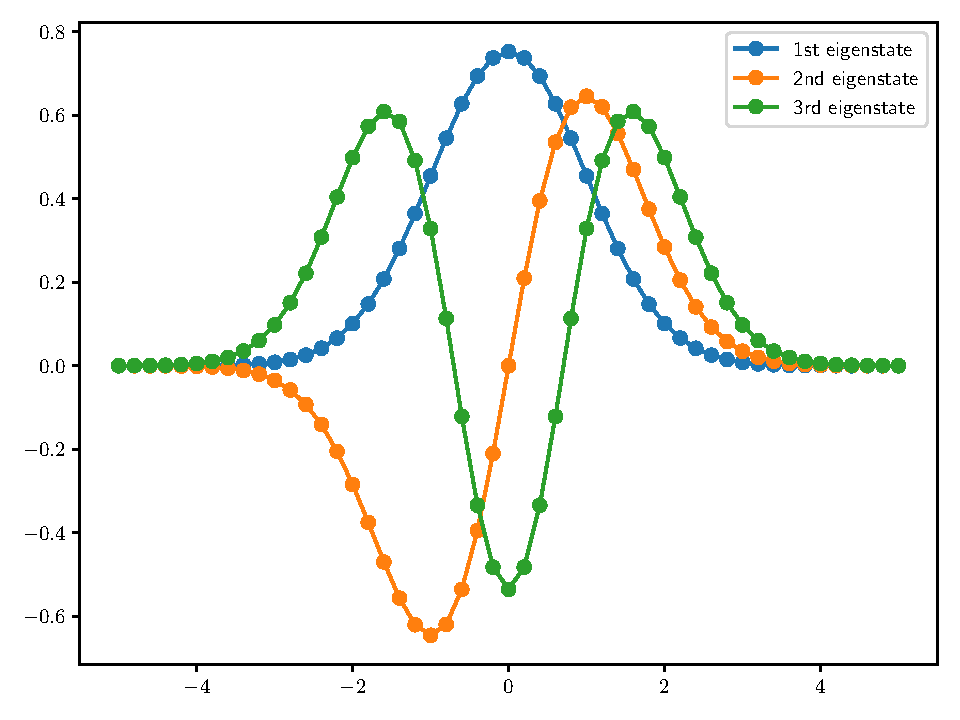
\includegraphics[width=0.6\textwidth]{../../codes/ks_dft_1d/IMG_main_harmonic_01_51.pdf}
\par}

Remember: eigenvectors are not unique.

\end{frame}


\begin{frame}
\frametitle{More about eigen}

Orbital energy levels:

Orbital filling, occupation number:

Total energy:

\end{frame}


\begin{frame}[fragile]
\frametitle{Some points regarding eigenvectors}

\begin{itemize}
\item Unlike eigenvalues, eigenvectors are not unique.
\item Eigenvectors forms orthonormal basis
\item In electronic structure calculations, we usually restrict eigenvectors to be
orthonormalized according to:
\begin{equation*}
\int_{-\infty}^{\infty} \psi^{*}_{i}(x) \psi_{j}(x) \, \mathrm{d}x = \delta_{ij}
\end{equation*}
\end{itemize}
We use the following to renormalize the eigenvectors:
\begin{juliacode}
for i in 1:3
    evecs[:,i] = evecs[:,i]/sqrt(dx)
end
\end{juliacode}

\end{frame}


\begin{frame}[fragile]
\frametitle{More accurate formulas for 2nd derivative}

\begin{itemize}
\item \jlinline{build_D2_matrix_3pt}
\item \jlinline{build_D2_matrix_5pt}
\item \jlinline{build_D2_matrix_7pt}
\item \jlinline{build_D2_matrix_9pt}
\item \jlinline{build_D2_matrix_11pt}
\end{itemize}

{\footnotesize \url{https://web.media.mit.edu/~crtaylor/calculator.html}}

\end{frame}


\begin{frame}[fragile]
\frametitle{Results (51 grid points, 11-points stencil for 2nd derivative)}

\begin{textcode}
Eigenvalues
State         Approx              Exact          Difference
   1       0.4999999996       0.5000000000   4.4949444167e-10
   2       1.4999999947       1.5000000000   5.2729647315e-09
   3       2.4999999782       2.5000000000   2.1831708441e-08
   4       3.5000000923       3.5000000000   9.2303385379e-08
   5       4.5000023627       4.5000000000   2.3626997363e-06
\end{textcode}

\end{frame}


\begin{frame}[fragile]
\frametitle{Let's try for another potential: attractive Gaussian potential}

$A$ and $\alpha$ are real, positive numbers.
$x_0$ is the center of the Gaussian.
\begin{equation*}
V(x) = -A \mathrm{e}^{-\alpha (x - x_0)^2}
\end{equation*}
This potential can be used to electron-ion interaction due to "atom" located
at $x_0$.

\begin{juliacode}
# assume A and α are positive numbers
function pot_gaussian( x; A=1.0, α=1.0, x0=0.0 )
    return -A*exp( -α*(x-x0)^2 )
end
\end{juliacode}

\end{frame}


\begin{frame}
\frametitle{Diatomic atom model}

Two Gaussians centered at $x = -1$ and $x = 1$.

\end{frame}



\begin{frame}
\frametitle{Calculate electron density}

Equation

\end{frame}


\begin{frame}
\frametitle{Hartree energy and potential}

\begin{align*}
E_{\mathrm{H}} & = \frac{1}{2} \int \int \frac{\rho(x) \rho(x')}{\left| x - x' \right|}\,\mathrm{d}x \mathrm{d}x' \\
& = \frac{1}{2} \int \rho(x) V_{\mathrm{H}}(x) \, \mathrm{d}x
\end{align*}
    
\begin{equation*}
V_{\mathrm{H}} = \int \frac{\rho(x')}{\left| x - x' \right|} \, \mathrm{d}x'
\end{equation*}

Approximating integral as sum:
\begin{equation*}
V_{\mathrm{H}}(x_{i}) \approx \sum_{j} \frac{\rho(x_{i})}{ \left| x_{i} - x_{j} \right| } \Delta x
\end{equation*}
This is divergent for $i = j$.

\end{frame}


\begin{frame}
\frametitle{Modification for Hartree potential}
    
To prevent singularity, we modify the Coulomb interaction:
\begin{equation*}
\frac{1}{\left| x - x' \right|} \rightarrow
\frac{1}{\sqrt{(x - x')^2 + a^2}}
\end{equation*}
where $a \neq 0$ is a parameter.

Our expression for the Hartree potential:
\begin{equation*}
V_{\mathrm{H}}(x_{i}) \approx \sum_{j} \frac{\rho(x_{i})}{\sqrt{ (x_{i} - x_{j})^2 + a^2 } } \Delta x
\end{equation*}

\end{frame}


\begin{frame}[fragile]
\frametitle{Solving for Hartree potential}

Direct sum (integration)

Code

\end{frame}


\begin{frame}
\frametitle{A sketch of self-consistent program}

Algorithm:

Schroedinger equation solver

Hartree potential calculation

\end{frame}


\begin{frame}
\frametitle{Electron density mixing}

Equation, code

\end{frame}



\end{document}
